\documentclass[letterpaper,12pt]{article}
\usepackage[utf8]{inputenc}
\usepackage[german]{babel}
\usepackage[right=2cm,left=4cm,top=1in,bottom=1in]{geometry}
\usepackage[dvipsnames]{xcolor}
%\\
\usepackage{mathrsfs}
\usepackage{amsmath}
\usepackage{amssymb}
\usepackage{latexsym}
\usepackage{pifont}
%\\
\usepackage{graphicx}
\usepackage{caption}
\usepackage[right]{sidecap}
% \\
\usepackage{fancyhdr}
\pagestyle{fancy}
\fancyhf{}
\lhead{Nadia Estefania Rosales Orozco}
\rhead{\textit{Seite \thepage}}
\lfoot{\small{4. November 2022}}
\rfoot{\small{Informatik für Physiker}}
%\\

\author{nadiarosaleso }
\date{November 2022}

\begin{document}
\begin{center}
    \textbf{\Large{Die Probleme}}
\end{center}

\section*{Probleme}
\begin{enumerate}
    \item {Betrachten Sie ein System in einer Dimension und wissen Sie, dass $a=\frac{dv}{dt}$ und $v=\frac{dx}{dt}$. Weisen Sie nach, dass die Position beschrieben werden kann als:}
\begin{equation*}
  {x=x_0+v_0t+\frac{1}{2}at^2}\hspace{1cm}
    \end{equation*}
Für einen Anfangszeitpunkt $t_0=0$ und mit; $x_0$ und 
$v_0$ die Anfangsposition und Geschwindigkeit im System.
\\Für $a = konstant$\hspace{1cm}$v=\frac{dx}{dt}$\hspace{1cm}$a=\frac{dv}{dt}$
\begin{align*}
    a=\frac{dv}{dt}\Rightarrow&\int^t_{t_0}{adt}=\int^t_{t_0}{\frac{dv}{dt}dt}\\
    durch\hspace{0.2cm}Variablenänderung\Rightarrow&a\int^t_{t_0}{dt}=\int^v_{v_0}{dv}\\
    \Rightarrow&at\Big|_{t_0}^t=v\Big|_{v_0}^{v}\\
     \Rightarrow&a(t-t_0)=v-v_0\\
     mit\hspace{0.4cm}t_0=0\Rightarrow&v=v_0+at\\
     \\
      v=\frac{dx}{dt}\Rightarrow&\int^t_{t_0}{vdt}=\int^t_{t_0}{\frac{dx}{dt}dt}\\
    durch\hspace{0.2cm}Variablenänderung\Rightarrow&\int^t_{t_0}{(v_0+at)dt}=\int^x_{x_0}{dx}\\
    \Rightarrow&v_0\int^t_{t_0}{dt}=a\int^t_{t_0}{tdt}=\int^x_{x_0}{dx}\\
    \Rightarrow&v_0t\Big|_{t_0}^t+a\frac{t^2}{2}\Big|_{t_0}^t=x\Big|_{x_0}^{x}\\
    \Rightarrow&v_0(t-t_0)+\frac{1}{2}a(t-t_0)^2=x-x_0\\
     mit\hspace{0.4cm}t_0=0\Rightarrow&x=x_0+v_0t+\frac{1}{2}at^2\\
\end{align*}
 \item {Betrachten Sie ein Rennen zwischen zwei Autos, sie starten aus dem Stand, Auto eins startet eine Sekunde vor Auto zwei, wenn die Autos eine Beschleunigung von 3,5 m/s2 und 4,9 m/s2 haben beziehungsweise.}
    \begin{enumerate}
        \item Zu welcher Zeit überholt Auto zwei Auto eins, i.e. t=?\\
        Sei ${x=x_0+v_0t+\frac{1}{2}at^2}$\hspace{0.5cm}, \hspace{0.5cm}$t_{A2}=t_f-1s$,\hspace{0.5cm}$x=\frac{1}{2}a_{A1}t_f^2$\hspace{0.5cm}und\\$x=\frac{1}{2}a_{A2}t_f^2=\frac{1}{2}a_{A2}(t_f-1s)^2$\\
        Dann setze x gleich und löse nach $t_f$ auf, wir haben:\\$t_{f}\approx6.45s$\hspace{0.2cm} und \hspace{0.2cm}$t_{C2}\approx5.45s$
        
        \item Was wird die Position sein, wenn Teil (a) auftritt, x =?\\
        Sei ${x=x_0+v_0t+\frac{1}{2}at^2}$\\
        Dann wird die Position zum Zeitpunkt $t_f$ sein:\\
        ${x=x_0+v_0t+\frac{1}{2}at^2}=\frac{1}{2}3.45\frac{m}{s^2}(6.45s)^2\approx72.8 m$
        
        \item Welche Geschwindigkeit wird es zu diesem Zeitpunkt für beide Autos haben?\\
        Sei $v=v_0+at$\\
        Dann wird die Geschwindigkeit zum Zeitpunkt $t_f$ sein:\\
        $v_{A1}=v_0+at=3.5\frac{m}{s^2}6.45s=22.57\frac{m}{s}$\\
        $v_{A2}=v_0+at=4.9\frac{m}{s^2}5.45s=26.70\frac{m}{s}$\\
        
        \item Nehmen Sie 5 verschiedene Zeiten ab, wann die Autos starten, ohne sich die Zeit zu nehmen Anfang, 3 vor dem Zeitpunkt, an dem sich die Autos treffen, und zwei danach Wetter. Erstellen Sie zwei Tabellen, eine für jedes Auto, mit den folgenden Informationen; Beschleunigung, Zeit, Position und Geschwindigkeit.\\Sehen Sie sich die Tabellen\ref{tab:my_label}.
    \end{enumerate}

\begin{table}[h]
    \centering
  \begin{tabular}{c|c|c|c}\hline\hline
 \multicolumn{4}{c}{Auto 1}\\\hline
 Nicht zeitabhängig &\multicolumn{3}{c}{Zeitabhängig}\\\hline
a[$\frac{m}{s^2}$] & t[s] & x[m] & v[$\frac{m}{s}$]\\\hline
\multirow{\centering
\begin{tabular}{c}
3.5\\
\end{tabular}} & 1 & 1.75 & 3.5 \\\cline{2-4}
 & 2 & 7 & 7 \\\cline{2-4}
 & 4 & 28 & 14\\\cline{2-4}
  & 7 & 85.75 & 24.5 \\\cline{2-4}
 & 10 & 175 & 35\\\hline\hline
\end{tabular}
    \caption{Kinematik von Auto 1}
    \label{tab:my_label}
\end{table}

\begin{table}[h]
    \centering
  \begin{tabular}{c|c|c|c}\hline\hline
 \multicolumn{4}{c}{Auto 2}\\\hline
 Nicht zeitabhängig &\multicolumn{3}{c}{Zeitabhängig}\\\hline
a[$\frac{m}{s^2}$] & t[s] & x[m] & v[$\frac{m}{s}$]\\\hline
\multirow{\centering
\begin{tabular}{c}
4.9\\
\end{tabular}} & 1 & 2.45 & 4.9 \\\cline{2-4}
 & 2 & 9.8 & 9.8 \\\cline{2-4}
 & 4 & 39.2 & 19.6\\\cline{2-4}
  & 7 & 120.05 & 34.3 \\\cline{2-4}
 & 10 & 245 & 49\\\hline\hline
\end{tabular}
    \caption{Kinematik von Auto 2}
    \label{tab:my_label}
\end{table}

    \item Betrachten Sie das folgende System, zwei Blöcke der Massen m1 und m2 werden durch verbunden eine ideale Saite und ruhen auf einer reibungsfreien horizontalen Oberfläche. Wenn eine Kraft der Größe A wird horizontal in der Richtung auf den Block der Masse m2 aufgebracht wie in Abbildung 1 gezeigt. Erstellen Sie die entsprechenden Freikörperdiagramme (verwenden Sie powerpoint, pait, zeichne es, was du willst) und hänge es als Bild an, aus Sie bestimmen die Beschleunigung des Systems und die Spannung der Saite zwischen den Blöcken.
     \begin{figure}[h]
        \caption{Freikörperbild des Systems.}
        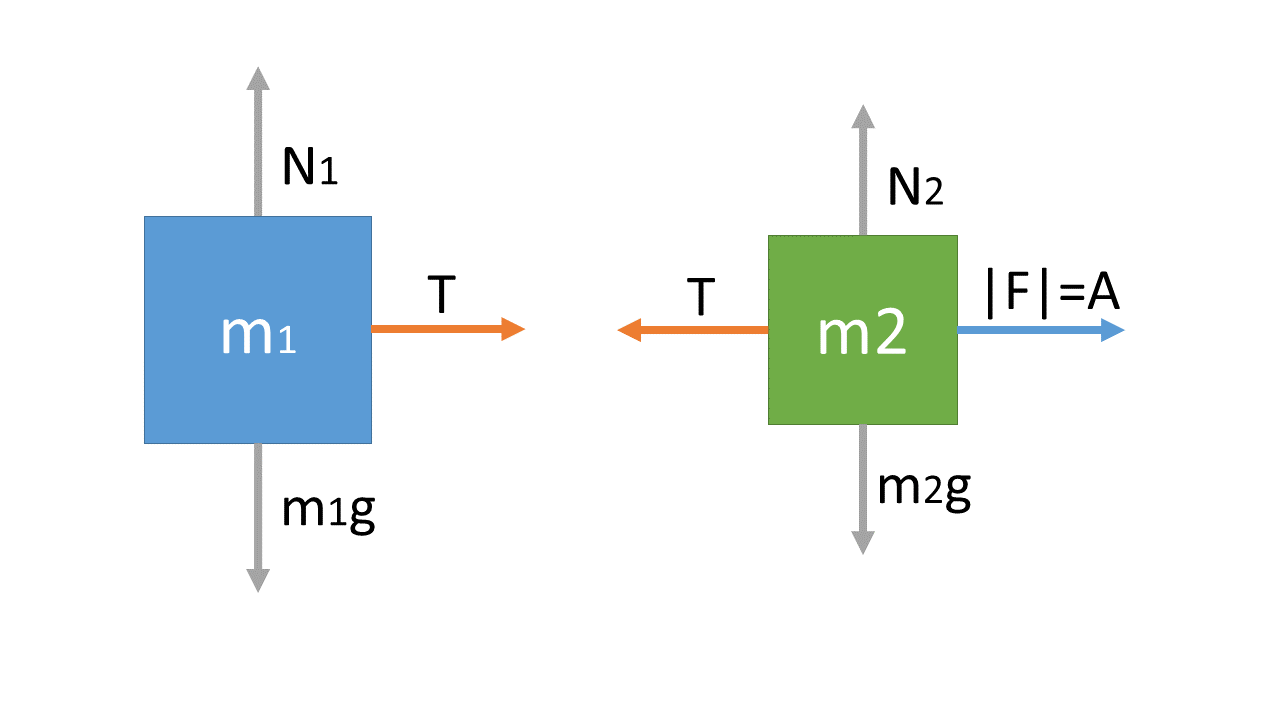
\includegraphics[scale=0.5]{Bildern/diagrama de cuerpo libre.png}
    \end{figure}\\
    Beachten Sie, dass die Spannung ist: $F=-T$\hspace{0.5cm} und da es keine Reibung gibt, dann ist die Kraft ist $F=(m1+m2)a$\hspace{0.2cm}also die Beschleunigung ist\hspace{0.2cm}$a=\frac{F}{(m1+m2)}$
\end{enumerate}


\end{document}
